\section{Nixtla Neural Forecast TimeGPT}
{{\footnotesize
\begin{description}[labelwidth=5em, labelsep=1em, leftmargin=*, align=left, itemsep=0.3em, parsep=0em]
  \item[date:] 2023-10-05
  \item[last\_updated:] 2025-06
  \item[expired:] unkown
  \item[valid:] yes
  \item[url:] \href{https://github.com/Nixtla/neuralforecast}{https://github.com/Nixtla/neuralforecast}
  \item[domain:] Time-series; General ML
  \item[focus:] Time-series foundation model "TimeGPT" for forecasting and anomaly detection
  \item[keywords:]
    - TimeGPT
    - foundation model
    - time-series
    - generative model
  \item[task\_types:]
    - Time-series forecasting
    - Anomaly detection
  \item[ai\_capability\_measured:]
    - Zero-shot forecasting
    - anomaly detection
  \item[metrics:]
    - RMSE
    - Anomaly detection metrics
  \item[models:]
    - TimeGPT
  \item[ml\_motif:]
    - Time-series
  \item[type:] Platform
  \item[ml\_task:] Forecasting
  \item[notes:] Offered via Nixtla API and Azure Studio; enterprise-grade support available.
  \item[contact.name:] Azul Garza (Nixtla)
  \item[contact.email:] unkown
  \item[results.name:] ChatGPT LLM
  \item[results.url:] \href{unkown}{unkown}
  \item[fair.reproducible:] Yes
  \item[fair.benchmark\_ready:] Yes
  \item[ratings.software.rating:] 0
  \item[ratings.software.reason:] Not analyzed.
  \item[ratings.specification.rating:] 7.0
  \item[ratings.specification.reason:] Describes forecasting with LLMs, but less formal on input/output or task framing.
  \item[ratings.dataset.rating:] 6.0
  \item[ratings.dataset.reason:] Uses open time series datasets, but lacks a consolidated data release or splits.
  \item[ratings.metrics.rating:] 7.0
  \item[ratings.metrics.reason:] Reports metrics like MASE and SMAPE, standard in forecasting.
  \item[ratings.reference\_solution.rating:] 6.0
  \item[ratings.reference\_solution.reason:] Provides TimeLLM with open source, but no other baselines included.
  \item[ratings.documentation.rating:] 6.0
  \item[ratings.documentation.reason:] GitHub readme with installation and example usage; lacks API or extensive tutorials.
  \item[id:] nixtla\_neural\_forecast\_timegpt
  \item[Citations:] \cite{garza2024timegpt1}
  \item[Ratings:]
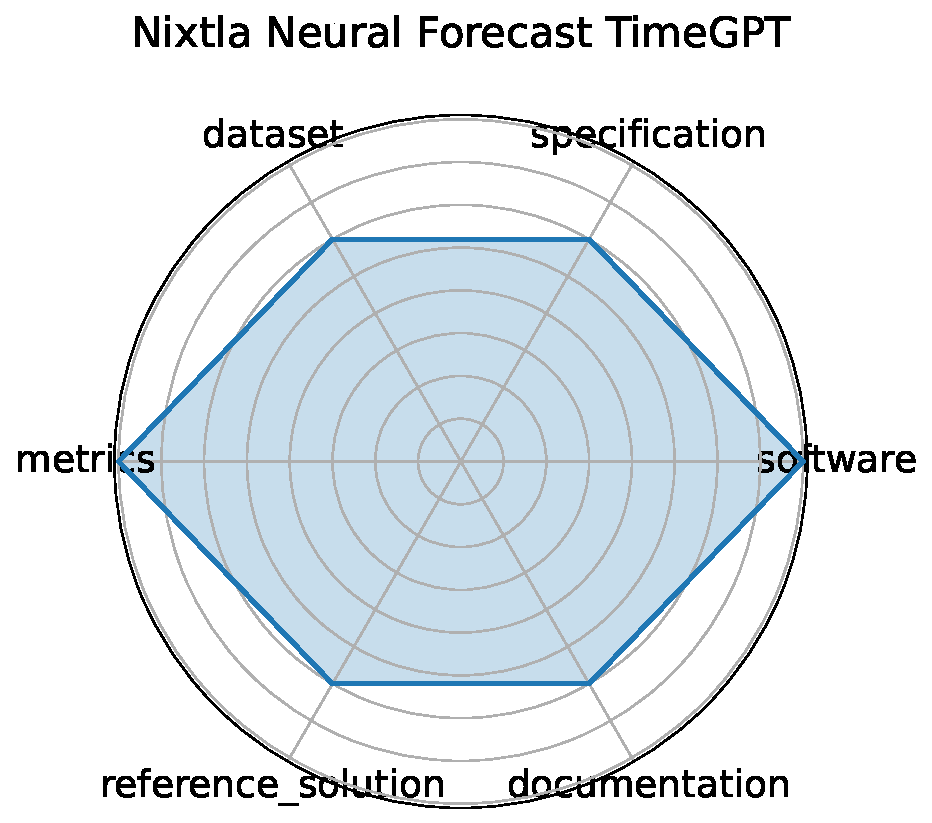
\includegraphics[width=0.2\textwidth]{nixtla_neural_forecast_timegpt_radar.pdf}
\end{description}
}}
\clearpage